\documentclass[cal1spr16Lectures.tex]{subfiles}

\begin{document}

\section[Week 4]{Week 4: 8-12 Feb}

% % %
\subsection[3.1 Introducing the Derivative]{\S 3.1 Introducing the Derivative}
% % %

% % %
\begin{frame}{\S 3.1 Introducing the Derivative}{}
{\bf Recall from Ch 2:}  We said that the slope of the tangent line at a point is the limit of the slopes of the secant lines as the points get closer and closer.
\begin{itemize}
\item slope of secant line:  $\dfrac{f(x)-f(a)}{x-a}$\ (average rate of change) 
\item slope of tangent line:  $\lim_{x \to a} \frac{f(x)-f(a)}{x-a}$\ (instantaneous rate of change)
\end{itemize}
\end{frame}

% % %
\begin{frame}
\centering{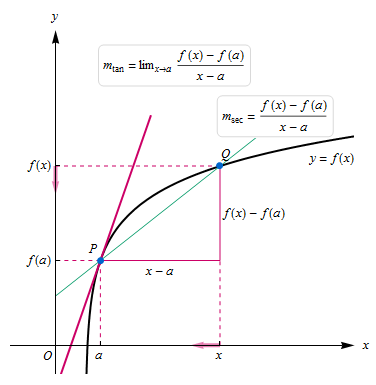
\includegraphics[scale=0.62]{pictures/lim}}
\end{frame}

% % %
\begin{frame}
\begin{exe} Use the relationship between secant lines and tangent lines, specifically the slope of the tangent line, to find the equation of a line tangent to the curve $f(x)=x^2+2x+2$ at the point $P=(1,5)$.
\end{exe}
\end{frame}

% % %
\begin{frame}{}
In the preceding exercise, we considered two points 
\vspace{-0.6pc}
\[P=\left(a,f(a)\right)\quad\text{and}\quad Q=\left(\alert{x},f(\alert{x})\right)\]
that were getting closer and closer together.

\vspace{2pc}
Instead of looking at the points approaching one another, we can also view this as the distance $h$ between the points approaching 0.  For 
\vspace{-0.5pc}
\[P=\left(a,f(a)\right)\quad\text{and}\quad Q=\left(\alert{a+h},f(\alert{a+h})\right),\]
\end{frame}

% % %
\begin{frame}
\begin{itemize}
\item slope of secant line:  
\[\frac{f(a+h)-f(a)}{(a+h)-a}= \dfrac{f(a+h)-f(a)}{h}\]
\item slope of tangent line:  
\[\lim_{h \to 0} \frac{f(a+h)-f(a)}{h}\]
\end{itemize}
\end{frame}

% % %
\begin{frame}
\centering{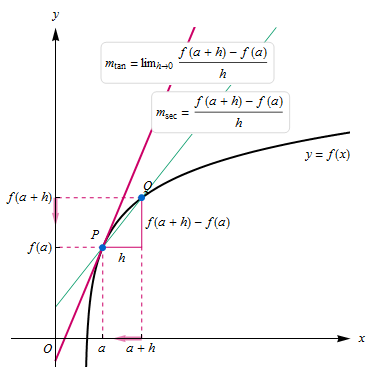
\includegraphics[scale=0.65]{pictures/limDef3_1}}
\end{frame}

% % %
\begin{frame}
\begin{exe} Find the equation of a line tangent to the curve $f(x)=x^2+2x+2$ at the point $P=(2,10)$. \end{exe}
\end{frame}

% % %
\subsubsection{Derivative Defined as a Function}
% % %

% % %
\begin{frame}{\small Derivative Defined as a Function}\footnotesize
The slope of the tangent line for the function $f$ is itself a function of $x$ (in other words, there is an expression where we can plug in any value $x=a$ and get the derivative at that point), called the derivative of $f$.
\begin{dfn} The {\bf derivative} of $f$ is the function 
\[f^{\prime}(x)=\lim_{h \to 0} \frac{f(x+h)-f(x)}{h},\]
provided the limit exists.  If $f^{\prime}(x)$ exists, we say $f$ is {\bf differentiable} at $x$.  If $f$ is differentiable at every point of an open interval $I$, we say that $f$ is differentiable on $I$. \end{dfn}
\end{frame}

% % %
\begin{frame}
\begin{exe} Use the definition of the derivative to find the derivative of the function $f(x)=x^2+2x+2$. \end{exe}
\end{frame}

% % %
\subsubsection{Leibniz Notation}
% % %

% % %
\begin{frame}{\small Leibniz Notation}
A standard notation for change involves the Greek letter $\Delta$. 
\[\frac{f(x+h)-f(x)}{h}=\frac{f(x+\Delta x)-f(x)}{\Delta x}=\frac{\Delta y}{\Delta x}.\]
Apply the limit:
\[f^{\prime}(x)=\lim_{\Delta x \to 0} \frac{f(x+\Delta x)-f(x)}{\Delta x}=\lim_{\Delta x \to 0} \frac{\Delta y}{\Delta x}=\alert{\frac{dy}{dx}}\]
\end{frame}

% % %
\subsubsection{Other Notation}
% % %

% % %
\begin{frame}{\small Other Notation}
The following are alternative ways of writing $f^{\prime}(x)$ (i.e., the derivative as a function of $x$):
\[\frac{dy}{dx}\qquad\frac{df}{dx} \qquad\frac{d}{dx}\left(f(x)\right) \qquad D_x (f(x)) \qquad y^{\prime}(x)\]
The following are ways to notate the derivative of $f$ evaluated at $x=a$:
\[f^{\prime}(a)\qquad y^{\prime}(a) \qquad \left. \frac{df}{dx} \right|_{x=a} \qquad \left. \frac{dy}{dx} \right|_{x=a}\]
\end{frame}

% % %
\begin{frame}
\begin{que}
Do the words ``derive" and ``differentiate" mean the same thing?
\end{que}
\end{frame}

% % %
\subsubsection{Graphing the Derivative}
% % %

% % %
\begin{frame}{\small Graphing the Derivative}
The graph of the derivative is the graph of the collection of slopes of tangent lines of a graph.  If you just have a graph (without an equation for the graph), the best you can do is approximate the graph of the derivative.
\end{frame}

% % %
\begin{frame}\footnotesize
\begin{ex}
\vspace{0.75pc}
\begin{columns}[T]
\begin{column}{0.45\textwidth}
	Simple checklist:
	\begin{itemize}
	\item[1.] Note where $f^{\prime}(x)=0$.
	\item[2.]  Note where $f^{\prime}(x)>0$.  (What does this look like?)
	\item[3.]  Note where $f^{\prime}(x)<0$.  (What does this look like?)
	\end{itemize}
\end{column}
\begin{column}{0.5\textwidth}	
	\centering{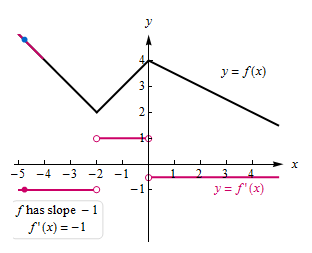
\includegraphics[scale=0.63]{pictures/graphDeriv3_1}}
\end{column}
\end{columns}
\end{ex}	
\end{frame}

% % %
\subsubsection{Differentiability vs. Continuity}
% % %

% % %
\begin{frame}{\small Differentiability vs. Continuity}
Key points about the relationship between differentiability and continuity:
\begin{itemize}
\item If $f$ is differentiable at $a$, then $f$ is continuous at $a$.
\item If $f$ is not continuous at $a$, then $f$ is not differentiable at $a$.
\item $f$ can be continuous at $a$, but not differentiable at $a$.
\end{itemize}
\end{frame}

% % %
\begin{frame}{}
A function $f$ is \alert{not} differentiable at $a$ if at least one of the following conditions holds:
\begin{itemize}
\item[1.] $f$ is not continuous at $a$.
\item[2.] $f$ has a corner at $a$.  
\begin{que} Why does this make $f$ not differentiable? \end{que}
\item[3.] $f$ has a vertical tangent at $a$.  
\begin{que} Why does this make $f$ not differentiable? \end{que}
\end{itemize}
\end{frame}

% % %
\subsubsection{Book Problems}
% % %

% % %
\begin{frame}
\begin{block}{3.1 Book Problems} 9-45 (odds), 49-53 (odds) \end{block}
\begin{itemize}
\item {\bf NOTE:}  You do not know any rules for differentiation yet (e.g., Power Rule, Chain Rule, etc.)  In this section, you are strictly using the definition of the derivative and the definition of slope of tangent lines we have derived.
\end{itemize}
\end{frame}

% % %
\subsection{Exam \#1 Review}
% % %

% % %
\begin{frame}[allowframebreaks]{Exam \#1 Review}\footnotesize
\begin{itemize}
\item $\oint$2.1  The Idea of Limits
	\begin{itemize}\footnotesize
	\item Understand the relationship between average velocity \& instantaneous velocity, and secant and tangent lines
	\item Be able to compute average velocities and use the idea of a limit to approximate instantaneous velocities
	\item Be able to compute slopes of secant lines and use the idea of a limit to approximate the slope of the tangent line
	\end{itemize}
\framebreak	
\item $\oint$2.2 Definitions of Limits
	\begin{itemize}\footnotesize
	\item Know the definition of a limit
	\item Be able to use a graph of a table to determine a limit
	\item Know the relationship between one- and two-sided limits
	\end{itemize}
\item $\oint$2.3 Techniques for Computing Limits
	\begin{itemize}\footnotesize
	\item Know and be able to compute limits using analytical methods (e.g., limit laws, additional techniques)
	\item Know the Squeeze Theorem and be able to use it to determine limits
	\end{itemize}
\framebreak
\begin{ex} Evaluate $\displaystyle\lim_{x\to 0}x\sin{\frac{1}{x}}$. \end{ex}	
\item $\oint$2.4 Infinite Limits
	\begin{itemize}\footnotesize
	\item Be able to use a graph, a table, or analytical methods to determine infinite limits
	\item Know the definition of a vertical asymptote  and be able to determine whether a function has vertical asymptotes 
	\end{itemize}
\framebreak
\item $\oint$2.5 Limits at Infinity
	\begin{itemize}\footnotesize
	\item Be able to find limits at infinity and horizontal asymptotes 
	\item Know how to compute the limits at infinity of rational functions
	\end{itemize}
\framebreak	
\begin{ex} Determine the end behavior of $f(x)$.  If there is a horizontal asymptote, then say so.  Next, identify any vertical asymptotes.  If $x=a$ is a vertical asymptote, then evaluate $\displaystyle\lim_{x\to a^+}f(x)$ and $\displaystyle\lim_{x\to a^-}f(x)$.
\[f(x)=\frac{2x^3+10x^2+12x}{x^3+2x^2}\]
\end{ex}
\framebreak
\item $\oint$2.6 Continuity 
	\begin{itemize}\footnotesize
	\item Know the definition of continuity and be able to apply the continuity checklist
	\item Be able to determine the continuity of a function (including those with roots) on an interval
	\item Be able to apply the Intermediate Value Theorem to a function
	\end{itemize}
\framebreak
\begin{ex} Determine the value for $a$ that will make $f(x)$ continuous. 
\[f(x)=\begin{cases}
	\frac{x^2+3x+2}{x+1} & x\neq -1 \\
	a & x=-1
	\end{cases}\]
\end{ex}
\begin{ex} Show that $f(x)=2$ has a solution on the interval $(-1,1)$, with
\[f(x)=2x^3+x.\]
\end{ex}
\framebreak
\item $\oint$2.7 Precise Definition of Limits 
	\begin{itemize}\footnotesize
	\item Understand the $\delta$, $\epsilon$ relationship for limits
	\item Be able to use a graph or analytical methods to find a value for $\delta>0$ given an $\epsilon>0$ (including finding symmetric intervals)
	\end{itemize}
\framebreak
\begin{ex}
\vspace{0.75pc}
\begin{columns}[T]
	\begin{column}{.25\textwidth}
	\centering{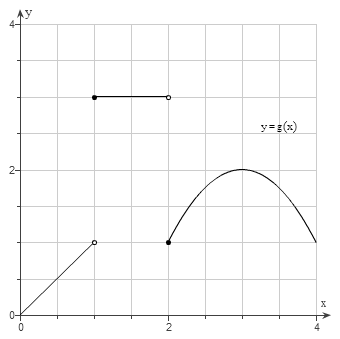
\includegraphics[scale=0.4]{pictures/Exam1pic}}
	\end{column}
	\begin{column}{.55\textwidth}
	Use the graph to find the appropriate $\delta$.
	\begin{itemize}\footnotesize
	\item[(a)]$|g(x)-2|<\textstyle\frac{1}{2}$ whenever 
	
	\hspace{6pc}$0<|x-3|<\delta$
	\item[(b)]$|g(x)-1|<\textstyle\frac{3}{2}$ whenever 
	
	\hspace{6pc}$0<|x-2|<\delta$
	\end{itemize}
	\end{column}
\end{columns}
\end{ex}
In this example, the two-sided limits at $x=1$ and $x=2$ do not exist.
\framebreak
\item $\oint$3.1 Introducing the Derivative
	\begin{itemize}\footnotesize
	\item Know the definition of a derivative and be able to use this definition to calculate the derivative of a given function
	\item Be able to determine the equation of a line tangent to the graph of a function at a given point
	\item Know the 3 conditions for when a function is not differentiable at a point, and why these three conditions make a function not differentiable at the given point
	\end{itemize}
\begin{ex}
	\begin{itemize}\footnotesize
	\item[(a)] Use the limit definition of the derivative to find an equation for the line tangent to $f(x)$ at $a$, where
	\[f(x)=\frac{1}{x};\quad a=-5.\]
	\item[(b)] Using the same $f(x)$ from part (a), find a formula for $f'(x)$ (using the limit definition).
	\item[(c)] Plug $-5$ into your answer for (b) and make sure it matches your answer for (a).
	\end{itemize}
\end{ex}
\end{itemize}
\end{frame}

% % %
\subsubsection{Other Study Tips}
% % %

% % %
\begin{frame}{\small Other Study Tips}\footnotesize
\begin{itemize}
\item Brush up on algebra, especially radicals.
%\item If your answer is something like $\sqrt 2$, don't plug that into your calculator, just leave it as is.
\item When in doubt, show steps.  Defer to class notes and old exams to get an idea of what's expected.
\item You will be punished for wrong notation; e.g., the limit symbol.
\item Read the question!  Several students always lose points because they didn't answer the question or they didn't follow directions.
\item Do the book problems.
%\item Look at the pictures in the book and the interactive applets on MLP.
\item Budget your time.  You don't have to do the problems in order.  Do the easier ones first.
\end{itemize}
\end{frame}

% % % 
\subsection[3.2 Rules of Differentiation]{$\textstyle\oint$3.2 Rules of Differentiation}
% % %

% % %
\begin{frame}{$\oint$3.2 Rules of Differentiation}
Recall the definition of the derivative:
\[f^{\prime}(x)=\lim_{h \to 0} \frac{f(x+h)-f(x)}{h}\]
(as a function of $x$, i.e., a formula).

And, for any particular point $a$, we have 
\[f^{\prime}(a)=\lim_{x \to a} \frac{f(x)-f(a)}{x-a}.\]
\end{frame}

% % %
\subsubsection{Constant Functions}
% % %

% % %
\begin{frame}{\small Constant Functions}\footnotesize
The constant function $f(x)=c$ is a horizontal line with a slope of 0 at every point.  This is consistent with the definition of the derivative:
\begin{align*}
f^{\prime}(x)&=\lim_{h \to 0} \frac{f(x+h)-f(x)}{h} \\
 &=\lim_{h \to 0} \frac{c-c}{h} \\[0.5pc]
 &=\lim_{h \to 0} 0 = 0.
\end{align*}
Therefore, for constant functions, \alert{$\frac{d}{dx}c=0$}.
\end{frame}

% % %
\subsubsection{Power Rule}
% % %

% % %
\begin{frame}{\small Power Rule}{}
{\bf Fact:} For any positive integer $n$, we can factor
\[x^n-a^n=(x-a)(x^{n-1}+x^{n-2}a+\cdots+xa^{n-2}+a^{n-1}).\]

For example, when $n=2$, we get
\[x^2-a^2=(x-a)(x+a),\]
which is the difference of squares formula.
\end{frame}

% % %
\begin{frame}{\small Power Rule, cont.}\footnotesize
Suppose $f(x)=x^n$ where $n$ is a positive integer.  Then at a point $a$,
\begin{align*}
f^{\prime}(a) &= \lim_{x \to a} \frac{f(x)-f(a)}{x-a} = \lim_{x \to a} \frac{x^n - a^n}{x-a} \\[0.25pc]
&= \lim_{x \to a} \frac{(x-a)(x^{n-1}+x^{n-2}a + \dots + xa^{n-2}+a^{n-1})}{x-a} \\[0.25pc]
&= (a^{n-1}+a^{n-2}\cdot a + \dots + a \cdot a^{n-2} + a^{n-1}) = n a^{n-1}. 
\end{align*}
Using the formula for the derivative as a function of $x$, one can show \alert{$\frac{d}{dx} (x^n)= nx^{n-1}$}.
\end{frame}

% % %
\subsubsection{Constant Multiple Rule}
% % %

% % %
\begin{frame}{\small Constant Multiple Rule}
Consider a function of the form $cf(x)$, where $c$ is a constant.  Just like with limits, we can factor out the constant: 
\begin{align*}
\frac{d}{dx}[cf(x)] &= \lim_{h \to 0} \frac{cf(x+h)-cf(x)}{h} \\
&= \lim_{h \to 0} \frac{c[f(x+h)-f(x)]}{h} = c\lim_{h \to 0} \frac{f(x+h)-f(x)}{h} \\[0.25pc]
&= cf^{\prime}(x)
\end{align*}
Therefore, \alert{$\frac{d}{dx}[cf(x)]=cf^{\prime}(x)$}.
\end{frame}

% % %
\subsubsection{Sum Rule}
% % %

% % %
\begin{frame}{\small Sum Rule}
Sums of functions also behave under the same limit laws when we differentiate:
\begin{align*}
\frac{d}{dx}[f(x)+g(x)] &= \lim_{h \to 0} \frac{[f(x+h)+g(x+h)]-[f(x)+g(x)]}{h} \\
&= \lim_{h \to 0} \left[\frac{[f(x+h)-f(x)]}{h}+\frac{[g(x+h)-g(x)]}{h}\right] \\[0.25pc]
&= \lim_{h \to 0} \frac{f(x+h)-f(x)}{h}+ \lim_{h \to 0}\frac{g(x+h)-g(x)}{h} \\[0.25pc]
&= f^{\prime}(x)+g^{\prime}(x)
\end{align*}
\end{frame}

% % %
\begin{frame}{}
So if $f$ and $g$ are differentiable at $x$,
\[\alert{\frac{d}{dx}[f(x)+g(x)]=f^{\prime}(x)+g^{\prime}(x)}.\]
The Sum Rule can be generalized for more than two functions to include $n$ functions.

\vspace{1pc}
{\bf Note:}  Using the Sum Rule and the Constant Multiple Rule produces the Difference Rule:
\[\alert{\frac{d}{dx}[f(x)-g(x)]=f^{\prime}(x)-g^{\prime}(x)}.\]
\end{frame}

% % %
\begin{frame}
\begin{exe}Using the differentiation rules we have discussed, calculate the derivatives of the following functions.  Note which rule(s) you are using.
\begin{itemize}
\item[1.] $y=x^5$
\item[2.] $y=4x^3-2x^2$
\item[3.] $y=-1500$
\item[4.] $y=3x^3-2x+4$
\end{itemize}
\end{exe}
\end{frame}

% % %
\subsubsection{Exponential Functions}
% % %

% % %
\begin{frame}{\small Exponential Functions}\footnotesize
Let $f(x)=b^x$, where $b>0$, $b \neq 1$.  To differentiate at $0$, we write
\[f^{\prime}(0)=\lim_{x \to 0}\frac{f(x)-f(0)}{x-0}=\lim_{x \to 0} \frac{b^x-b^0}{x}=
\lim_{x \to 0} \frac{b^x-1}{x}.\]

\vspace{1pc}
It is not obvious what this limit should be.  However, consider the cases $b=2$ and $b=3$.  By constructing a table of values, we can see that 
\[\lim_{x \to 0} \frac{2^x-1}{x} \approx 0.693 \quad \text{and}\quad \lim_{x \to 0} \frac{3^x-1}{x} \approx 1.099.\]
\end{frame}

% % %
\begin{frame}\footnotesize
So, $f^{\prime}(0)<1$ when $b=2$ and $f^{\prime}(0)>1$ when $b=3$.  As it turns out, there is a particular number $b$, with $2<b<3$, whose graph has a tangent line with slope 1 at $x=0$.  In other words, such a number $b$ has the property that 
\[\lim_{x \to 0} \frac{b^x-1}{x}=1.\]
\begin{que}What number is it? \end{que}
{\bf Answer:} This number is $e=2.718281828459 \dots$ (known as the Euler number).  The function $f(x)=e^x$ is called the \alert{\bf natural exponential function}.
\end{frame}

% % % 
\begin{frame}\footnotesize
Now, using  $\displaystyle\lim_{x \to 0} \frac{e^x-1}{x}=1$, we can find the formula for $\frac{d}{dx}(e^x)$:
\begin{align*}
\alert{\frac{d}{dx}(e^x)} &= \lim_{h \to 0} \frac{e^{x+h}-e^x}{h} \\[0.25pc]
 &= \lim_{h \to 0}\frac{e^x \cdot e^h -e^x}{h} \\[0.25pc]
 &= \lim_{h\to 0}\frac{e^x(e^h-1)}{h} \\[0.25pc]
 &=e^x \left(\lim_{h \to 0} \frac{e^h-1}{h}\right) \\[0.25pc]
  &= e^x \cdot 1 = \alert{e^x}
\end{align*}
\end{frame}

% % %
\begin{frame}{}
\begin{exe} 
	\begin{itemize}
	\item[(a)] Find the slope of the line tangent to the curve $f(x)=x^3-4x-4$ at the point $(2,-4)$. 
	\item[(b)] Where does this curve have a horizontal tangent?
	\end{itemize}
\end{exe}	
\end{frame}

% % %
\subsubsection{Higher-Order Derivatives}
% % %

% % %
\begin{frame}{\small Higher-Order Derivatives}
If we can write the derivative of $f$ as a function of $x$, then we can take \emph{its} derivative, too.  The derivative of the derivative is called the {\bf second derivative} of $f$, and is denoted $f^{\prime\prime}$.  

\vspace{1pc}
In general, we can differentiate $f$ as often as needed.  If we do it $n$ times, the $n$th derivative of $f$ is 
\[\alert{f^{(n)}}(x)=\frac{\alert{d^n} f}{\alert{dx^n}}=\alert{\frac{d}{dx}}[\alert{f^{(n-1)}}(x)].\]
\end{frame}

% % %
\subsubsection{Book Problems}
% % %

% % %
\begin{frame}{}
\begin{block}{3.2 Book Problems} 3-45 (x3) \end{block} 
\begin{itemize}
\item For these problems, use only the rules we have derived so far.
\end{itemize}
\end{frame}

% % %
\subsection[3.3 The Product and Quotient Rules]{$\textstyle\oint$3.3 The Product and Quotient Rules}
% % %

% % %
\begin{frame}{$\oint$3.3 The Product and Quotient Rules}
Issue: Derivatives of products and quotients do \alert{NOT} behave like they do for limits.  
\end{frame}

% % %
\begin{frame}\footnotesize
As an example, consider $f(x)=x^2$ and $g(x)=x^3$.  We can try to differentiate their product in two ways:
\begin{itemize}\footnotesize
\item $\begin{aligned}[t]
	\frac{d}{dx}[f(x)g(x)] &= \frac{d}{dx}\left(x^5 \right) \\[0.25pc]
	 &= 5x^4
	\end{aligned}$
\item $\begin{aligned}[t]
	f^{\prime}(x)g^{\prime}(x) &= (2x)(3x^2) \\
	 &= 6x^3
	 \end{aligned}$
\end{itemize}
\begin{que}Which answer is the correct one? \end{que}
\end{frame}

% % %
\subsubsection{Product Rule}
% % %

% % %
\begin{frame}{\small Product Rule}\footnotesize
If $f$ and $g$ are any two functions that are differentiable at $x$, then
\[\alert{\frac{d}{dx}[f(x) g(x)] = f^{\prime}(x) g(x) + g^{\prime}(x) f(x)}.\]
In the example from the previous slide, we have
\begin{align*}
\frac{d}{dx}[x^2\cdot x^3] &= \frac{d}{dx}(x^2)\cdot (x^3)+x^2\cdot\frac{d}{dx}(x^3) \\
 &= (2x)\cdot (x^3)+x^2\cdot (3x^2) \\[0.25pc]
 &= 2x^4+3x^4 \\[0.25pc]
 &= 5x^4
\end{align*}
\end{frame}

% % %
\subsubsection{Derivation of the Product Rule}
% % %

% % %
\begin{frame}[allowframebreaks]{\small Derivation of the Product Rule}\footnotesize
\begin{align*}
&\frac{d}{dx}[f(x)g(x)] = \lim_{h \to 0} \frac{f(x+h)g(x+h)-f(x)g(x)}{h} \\[1pc]
 =\lim_{h \to 0} &\left(\frac{f(x+h)g(x+h)+\alert{[-f(x)g(x+h)+f(x)g(x+h)]}-f(x)g(x)}{h}\right) \\[0.5pc] 
 =\lim_{h \to 0} &\left(\frac{f(x+h)g(x+h)\alert{-f(x)g(x+h)}}{h}\right) \\
&\hspace{5pc} + \left(\lim_{h \to 0}\frac{\alert{f(x)g(x+h)}-f(x)g(x)}{h}\right) \\[0.5pc]
\end{align*} 

\framebreak
\begin{align*} 
 =\lim_{h \to 0} &\left(g(x+h) \frac{f(x+h)-f(x)}{h}\right) + \left(\lim_{h \to 0} f(x) \frac{g(x+h)-g(x)}{h}\right) \\[0.5pc]
 &=g(x)f^{\prime}(x)+f(x)g^{\prime}(x)
\end{align*}
\end{frame}

% % %
\subsubsection{Derivation of the Quotient Rule}
% % %

% % %
\begin{frame}{\small Derivation of Quotient Rule}\footnotesize
\begin{que} Let $q(x)=\frac{f(x)}{g(x)}$.  What is $\frac{d}{dx}q(x)$? \end{que}
{\bf Answer:} We can write $f(x)=q(x) g(x)$ and then use the Product Rule:
\[f^{\prime}(x) = q^{\prime}(x) g(x) + g^{\prime}(x) q(x)\] 
and now solve for $q^{\prime}(x)$: 
\[q^{\prime}(x)=\frac{f^{\prime}(x)-q(x)g^{\prime}(x)}{g(x)}.\]
\end{frame} 

% % %
\begin{frame}{}\footnotesize
Then, to get rid of $q(x)$, plug in $\frac{f(x)}{g(x)}$:
\begin{align*}
q^{\prime}(x) &= \frac{f^{\prime}(x)-g^{\prime}(x)\alert{\frac{f(x)}{g(x)}}}{g(x)} \\[0.5pc]
 &= \frac{\alert{g(x)} \left( f^{\prime}(x)-g^{\prime}(x)\frac{f(x)}{g(x)} \right)}{\alert{g(x)}\cdot g(x)} \\[1pc]
\alert{\frac{d}{dx}\left(\frac{f(x)}{g(x)}\right)} & \alert{=\frac{f^{\prime}(x) g(x)-g^{\prime}(x)f(x)}{g(x)^2}}
\end{align*}
``LO-D-HI minus HI-D-LO  over LO squared"
\end{frame}

% % %
\subsubsection{Quotient Rule}
% % %

% % % 
\begin{frame}{\small Quotient Rule}
Just as with the product rule, the derivative of a quotient is not a quotient of derivatives, i.e.
\[\frac{d}{dx} \left[ \frac{f(x)}{g(x)}\right] \ne \frac{f^{\prime}(x)}{g^{\prime}(x)}.\]
Here is the correct rule, the Quotient Rule:
\[\frac{d}{dx} \left[ \frac{f(x)}{g(x)}\right] = \frac{f^{\prime}(x) g(x)-g^{\prime}(x) f(x)}{[g(x)]^2}.\]
\end{frame}

% % %
\begin{frame}
\begin{exe} Use the Quotient Rule to find the derivative of 
\[\frac{4x^3+2x-3}{x+1}.\]
\end{exe}
\begin{exe} Find the slope of the tangent line to the curve 
\[f(x)=\frac{2x-3}{x+1}\text{ at the point }(4,1).\] 
\end{exe}
\end{frame}

% % %
\begin{frame}{}
The Quotient Rule also allows us to extend the Power Rule to negative numbers -- if $n$ is any integer, then 
\[\frac{d}{dx}\left[ x^n \right] = nx^{n-1}.\]
\begin{que} How? \end{que}
\end{frame}

% % %
\begin{frame}
\begin{exe} If $f(x)=\frac{x(3-x)}{2x^2}$, find $f^{\prime}(x).$ \end{exe}
\end{frame}

% % %
\subsubsection{Derivative of $e^{kx}$}
% % %

% % %
\begin{frame}{\small Derivative of $e^{kx}$}
For any real number $k$,
\[\frac{d}{dx} \left( e^{kx} \right) = ke^{kx}.\]
\begin{exe}What is the derivative of $x^2 e^{3x}$? \end{exe}
\end{frame}

% % %
\subsubsection{Rates of Change}
% % %

% % %
\begin{frame}{\small Rates of Change}\footnotesize
The derivative provides information about the instantaneous rate of change of the function being differentiated (compare to the limit of the slopes of the secant lines from $\textstyle\oint$2.1).

\vspace{1pc}
For example, suppose that the population of a culture can be modeled by the function $p(t)$.  We can find the instantaneous growth rate of the population at any time $t \ge 0$ by computing $p^{\prime}(t)$ as well as the \alert{\bf steady-state population} (also called the {\bf carrying capacity} of the population).  The steady-state population equals 
\[\lim_{t \to \infty} p(t).\]
\end{frame}

% % %
\subsubsection{Book Problems}
% % %

% % %
\begin{frame}{}
\begin{block}{3.3 Book Problems} 6-51 (x3) \end{block} 
\end{frame}

% % %
\subsection[3.4 Derivatives of Trigonometric Functions]{$\textstyle\oint$3.4 Derivatives of Trigonometric Functions}
% % %

% % %
\begin{frame}{$\oint$3.4 Derivatives of Trigonometric Functions}
Derivative formulas for sine and cosine can be derived using the following limits:
\begin{itemize}
	\item $\lim_{x \to 0} \frac{\sin x}{x}=1$
	\item $\lim_{x \to 0} \frac{\cos x -1}{x}=0$
\end{itemize}
(We will prove these limits in Chapter 4.)
\end{frame}

% % %
\begin{frame}
\begin{exe} Evaluate $\displaystyle\lim_{x \to 0} \frac{\sin 9x}{x}$ and $\displaystyle\lim_{x \to 0} \frac{\sin 9x}{\sin 5x}.$ \end{exe}
\end{frame}

% % %
\subsubsection{Derivatives of Sine and Cosine Functions}
% % %

% % %
\begin{frame}{\small Derivatives of Sine and Cosine Functions}
Using the previous limits and the definition of the derivative, we obtain
\begin{align*}
\frac{d}{dx} (\sin x) &= \cos x \\
\frac{d}{dx} (\cos x) &= -\sin x
\end{align*}
\end{frame}

% % %
\subsubsection{Trig Identities You Should Know}
% % %

% % %
\begin{frame}{\small Trig Identities You Should Know}
\begin{columns}[T]
\begin{column}{.5\textwidth}
\begin{itemize}\footnotesize
	\item $\sin^2 x + \cos^2 x = 1$ \vspace{0.2cm}
	\item $\tan^2 x + 1 = \sec^2 x$ \vspace{0.2cm}
	\item $\sin 2x =2\sin x \cos x$ \vspace{0.2cm}
	\item $\cos 2x = 1-2\sin^2 x$ \vspace{0.2cm}
	\item $\cos^2 x = \frac{1+\cos 2x}{2}$ \vspace{0.1cm}
	\item $\sin^2 x = \frac{1-\cos 2x}{2}$ \vspace{0.2cm}
\end{itemize}
\end{column}
\begin{column}{.5\textwidth}
\begin{itemize}\footnotesize
	\item $\tan x = \frac{\sin x}{\cos x}$ \vspace{0.2cm}
	\item $\cot x = \frac{\cos x}{\sin x}$ \vspace{0.2cm}
	\item $\cot x = \frac{1}{\tan x}$ \vspace{0.2cm}
	\item $\sec x = \frac{1}{\cos x}$ \vspace{0.1cm}
	\item $\csc x = \frac{1}{\sin x}$ \vspace{0.2cm}
\end{itemize}
\end{column}
\end{columns}
\end{frame}

% % %
\subsubsection{Derivatives of Other Trig Functions}
% % %

% % %
\begin{frame}{\small Derivatives of Other Trig functions}\footnotesize
\begin{align*}
\frac{d}{dx}(\tan x)&=\frac{d}{dx} \left( \frac{\sin x}{\cos x}\right) \\
 &= \frac{\cos x \cos x - (-\sin x)\sin x }{\cos^2 x} \\
&= \frac{\cos^2 x + \sin^2 x}{\cos^2 x} \\
&= \frac{1}{\cos^2 x} = \sec^2 x
\end{align*}
So \alert{$\frac{d}{dx} (\tan x)=\sec^2 x$}.
\end{frame}

% % %
\begin{frame}{}
By using trig identities and the Quotient Rule, we obtain
\begin{align*}
\alert{\frac{d}{dx} (\csc x)} &= \frac{d}{dx} \left( \frac{1}{\sin x}\right) = \alert{-\csc x \cot x} \\
\alert{\frac{d}{dx} (\sec x)} &= \frac{d}{dx} \left( \frac{1}{\cos x}\right) = \alert{\sec x \tan x} \\
\alert{\frac{d}{dx} (\cot x)} &= \frac{d}{dx} \left( \frac{1}{\tan x}\right) = \alert{-\csc^2 x}  
\end{align*}
\end{frame}

% % %
\begin{frame}
\begin{exe} Compute the derivative of the following functions:
\[f(x)=\frac{\tan x}{1+\tan x} \qquad g(x)=\sin x \cos x\]
\end{exe}
\end{frame}

% % %
\subsubsection{Higher-Order Trig Derivatives}
% % %

% % %
\begin{frame}{\small Higher-Order Trig Derivatives}
There is a cyclic relationship between the higher order derivatives of $\sin x$ and $\cos x$:
\begin{columns}
\begin{column}{.45\textwidth}
\[\begin{split}
	f(x) &=\sin x \\  
	f^{\prime}(x) &=\cos x \\
	f^{\prime\prime}(x) &=-\sin x \\
	f^{(3)}(x) &=-\cos x \\
	f^{(4)}(x) &=\sin x 
\end{split}\]
\end{column}
\begin{column}{.6\textwidth}
\[\begin{split}
	g(x) &=\cos x \\
	g^{\prime}(x) &=-\sin x \\
	g^{\prime\prime}(x) &=-\cos x \\
	g^{(3)}(x) &=\sin x \\
	g^{(4)}(x) &=\cos x 
\end{split}\]
\end{column}
\end{columns}
\end{frame}

% % %
\subsubsection{Book Problems}
% % %

% % %
\begin{frame}
\begin{block}{3.4 Book Problems} 7, 13, 17, 21-27, 33, 35, 44-46, 53-55 \end{block} 
\end{frame}

% % %
\subsection[3.5 Derivatives as Rates of Change]{$\textstyle\oint$3.5 Derivatives as Rates of Change}
% % %

% % %
\begin{frame}{$\oint$3.5 Derivatives as Rates of Change}{\fontsize{11}{12}\selectfont Position and Velocity}
Suppose an object moves along a straight line and its location at time $t$ is given by the position function $s=f(t)$.  The {\bf displacement} of the object between $t=a$ and $t=a+\Delta t$ is 
\[\Delta s = f(a+\Delta t)-f(a).\]
Here $\Delta t$ represents how much time has elapsed.
\end{frame}

% % %
\begin{frame}{}
We now define average velocity as 
\[\frac{\Delta s}{\Delta t}=\frac{f(a+\Delta t)-f(a)}{\Delta t}.\]
Recall that the limit of the average velocities as the time interval approaches 0 was the instantaneous velocity (which we denote here by $v$).  Therefore, the instantaneous velocity at $a$ is 
\[v(a)=\lim_{\Delta t \to 0} \frac{f(a+\Delta t)-f(a)}{\Delta t} = f^{\prime}(a).\]
\end{frame}

% % %
\begin{frame}{}
In mathematics, speed and velocity are related but not the same -- if the \alert{velocity} of an object at any time $t$ is given by $v(t)$, then the \alert{speed} of the object at any time $t$ is given by 
\[|v(t)|=|f^{\prime}(t)|.\]
\end{frame}

% % %
\begin{frame}[allowframebreaks]{}
By definition, acceleration (denoted by $a$) is the instantaneous rate of change of the velocity of an object at time $t$.  Therefore,
\[a(t)=v^{\prime}(t)\]
and since velocity was the derivative of the position function $s=f(t)$, then 
\[a(t)=v^{\prime}(t)=f^{\prime\prime}(t).\]

\framebreak
{\bf Summary:}  Given the position function $s=f(t)$, the velocity at time $t$ is the first derivative, the speed at time $t$ is the absolute value of the first derivative, and the acceleration at time $t$ is the second derivative.
\end{frame}

% % %
\begin{frame}
\begin{que} Given the position function $s=f(t)$ of an object launched into the air, how would you know:
\begin{itemize}
	\item The highest point the object reaches?
	\item How long it takes to hit the ground?
	\item The speed at which the object hits the ground?
\end{itemize}
\end{que}
\end{frame}

% % %
\subsubsection{Growth Models}
% % %

% % %
\begin{frame}{\small Growth Models}
Suppose $p=f(t)$ is a function of the growth of some quantity of interest.  The average growth rate of $p$ between times $t=a$ and a later time $t=a+\Delta t$ is the change in $p$ divided by the elapsed time $\Delta t$:
\[\frac{\Delta p}{\Delta t}=\frac{f(a+\Delta t)-f(a)}{\Delta t}.\]
\end{frame}

% % %
\begin{frame}{}
As $\Delta t$ approaches 0, the average growth rate approaches the derivative $\frac{dp}{dt}$, which is the instantaneous growth rate (or just simply the growth rate).  Therefore,
\[\frac{dp}{dt}=\lim_{\Delta t \to 0} \frac{f(a+\Delta t)-f(a)}{\Delta t} = \lim_{\Delta t \to 0} \frac{\Delta p}{\Delta t}.\]
\end{frame}

% % %
\begin{frame}
\begin{exe} The population of the state of Georgia (in thousands) from 1995 ($t=0$) to 2005 ($t=10$) is modeled by the polynomial 
\[p(t)=-0.27t^2+101t+7055.\]
\begin{itemize}
	\item[(a)] What was the average growth rate from 1995 to 2005?
	\item[(b)] What was the growth rate for Georgia in 1997?
	\item[(c)] What can you say about the population growth rate in Georgia between 1995 and 2005?
\end{itemize}
\end{exe}
\end{frame}

% % %
\subsubsection{Average and Marginal Cost}
% % %

% % %
\begin{frame}{\small Average and Marginal Cost}
Suppose a company produces a large amount of a particular quantity.  Associated with manufacturing the quantity is a {\bf cost function} $C(x)$ that gives the cost of manufacturing $x$ items.  This cost may include a {\bf fixed cost} to get started as well as a {\bf unit cost} (or {\bf variable cost}) in producing one item.
\end{frame}

% % %
\begin{frame}{}
If a company produces $x$ items at a cost of $C(x)$, then the average cost is $\frac{C(x)}{x}.$  This average cost indicates the cost of items already produced.  Having produced $x$ items, the cost of producing another $\Delta x$ items is $C(x+\Delta x)-C(x)$.  So the average cost of producing these extra $\Delta x$ items is 
\[\frac{\Delta C}{\Delta x}=\frac{C(x+\Delta x)-C(x)}{\Delta x}.\]
\end{frame}

% % %
\begin{frame}{}
If we let $\Delta x$ approach 0, we have
\[\lim_{\Delta x \to 0}\frac{\Delta C}{\Delta x}=C^{\prime}(x)\]
which is called the {\bf marginal cost}.  The marginal cost is the approximate cost to produce one additional item after producing $x$ items.

\vspace{1pc}
{\bf Note:}  In reality, we can't let $\Delta x$ approach 0 because $\Delta x$ represents whole numbers of items.
\end{frame}

% % %
\begin{frame}
\begin{exe} If the cost of producing $x$ items is given by 
\[C(x)=-0.04x^2+100x+800\]
for $0 \le x \le 1000$, find the average cost and marginal cost functions.  Also, determine the average and marginal cost when $x=500.$ \end{exe}
\end{frame}

% % %
\subsubsection{Book Problems}
% % %

% % %
\begin{frame}
\begin{block}{3.5 Book Problems} 9-12, 17-18, 22-23, 27-37 (odds) \end{block}
\end{frame}

% % %
\subsection[3.6 The Chain Rule]{$\textstyle\oint$3.6 The Chain Rule}
% % %

% % %
\begin{frame}{$\oint$3.6 The Chain Rule}\footnotesize
Suppose that Yvonne ($y$) can run twice as fast as Uma ($u$). Therefore $\frac{dy}{du}=2$.

\vspace{1pc}
Suppose that Uma can run four times as fast as Xavier ($x$).  So $\frac{du}{dx}=4$.

\vspace{1pc}
How much faster can Yvonne run than Xavier?  In this case, we would take both our rates and multiply them together:
\[\frac{dy}{du} \cdot \frac{du}{dx}=2 \cdot 4 = 8.\]
\end{frame}

% % % 
\subsubsection{Version 1 of the Chain Rule}
% % %

% % %
\begin{frame}{\small Version 1 of the Chain Rule}
If $g$ is differentiable at $x$, and $y=f(u)$ is differentiable at $u=g(x)$, then the composite function $y=f(g(x))$ is differentiable at $x$, and its derivative can be expressed as 
\[\frac{dy}{dx}=\frac{dy}{du} \cdot \frac{du}{dx}\]
\end{frame}

% % %
\subsubsection{Guidelines for Using the Chain Rule}
% % %

% % %
\begin{frame}{\small Guidelines for Using the Chain Rule}\footnotesize
Assume the differentiable function $y=f(g(x))$ is given.
\begin{itemize}
	\item[1.] Identify the outer function $f$, the inner function $g$, and let $u=g(x).$
	\item[2.] Replace $g(x)$ by $u$ to express $y$ in terms of $u$:
	\[y=f(g(x)) \implies y=f(u)\]
	\item[3.]  Calculate the product $\frac{dy}{du} \cdot \frac{du}{dx}$
	\item[4.] Replace $u$ by $g(x)$ in $\frac{dy}{du}$ to obtain $\frac{dy}{dx}.$
\end{itemize}
\end{frame}

% % %
\begin{frame}\footnotesize
\begin{ex} Use Version 1 of the Chain Rule to calculate $\frac{dy}{dx}$ for $y=(5x^2 +11x)^{20}$. \end{ex}
\begin{itemize}
\item inner function: $u=5x^2+11x$ 
\item outer function: $y=u^{20}$
\end{itemize}

\vspace{1pc}
We have $y = f(g(x)) = (5x^2 +11x)^{20}$.  Differentiate:
\begin{align*} 
\frac{dy}{dx}= \frac{dy}{du}\cdot\frac{du}{dx} &= 20u^{19} \cdot (10x+11) \\
 &=20(5x^2 +11x)^{19} \cdot (10x+11)
\end{align*}
\end{frame}

% % %
\begin{frame}
\begin{exe} Use the first version of the Chain Rule to calculate $\frac{dy}{dx}$ for 
\[y=\left( \frac{3x}{4x+2} \right)^5.\]
\end{exe}
\end{frame}

% % %
\subsubsection{Version 2 of the Chain Rule}
% % %

% % %
\begin{frame}{\small Version 2 of the Chain Rule}
Notice if $y=f(u)$ and $u=g(x)$, then $y=f(u)=f(g(x))$, so we can also write:
\begin{align*}
\frac{dy}{dx} &= \frac{dy}{du} \cdot \frac{du}{dx} \\[0.75pc]
 &= f^{\prime}(u) \cdot g^{\prime}(x) \\[0.75pc]
 &= f^{\prime}(g(x)) \cdot g^{\prime}(x).
\end{align*}
\end{frame}

% % %
\begin{frame}\footnotesize
\begin{ex} Use Version 2 of the Chain Rule to calculate $\frac{dy}{dx}$ for $y=(7x^4+2x+5)^9$. \end{ex}
\begin{itemize}
\item inner function: $g(x)=7x^4+2x+5$ 
\item outer function: $f(u)=u^9$
\end{itemize}
Then
\begin{align*}
f^{\prime}(u) &= 9u^8 \implies f^{\prime}(g(x))=9(7x^4+2x+5)^8 \\
g^{\prime}(x) &=28x^3+2.
\end{align*}
Putting it together,
\[\frac{dy}{dx}=f^{\prime}(g(x)) \cdot g^{\prime}(x) = 9(7x^4+2x+5)^8 \cdot (28x^3+2)\]
\end{frame}

% % %
\subsubsection{Chain Rule for Powers}
% % %

% % % 
\begin{frame}[allowframebreaks]{\small Chain Rule for Powers}
If $g$ is differentiable for all $x$ in the domain and $n$ is an integer, then
\[\frac{d}{dx} \bigg[\left(g(x)\right)^n \bigg]=n(g(x))^{n-1} \cdot g^{\prime}(x).\]

\framebreak
\begin{ex} $\frac{d}{dx} \bigg[ (1-e^x)^4 \bigg] =$ ? \end{ex}
{\bf Answer:}
\begin{align*}
\frac{d}{dx} \bigg[ (1-e^x)^4 \bigg] &= 4(1-e^x)^3 \cdot (-e^x) \\
 &= -4e^x (1-e^x)^3
\end{align*}
\end{frame}

% % %
\subsubsection{Composition of 3 or More Functions}
% % %

% % %
\begin{frame}[allowframebreaks]{\small Composition of 3 or More Functions}
\begin{ex}Compute $\frac{d}{dx} \bigg[ \sqrt{(3x-4)^2 + 3x} \bigg]$. \end{ex}

\framebreak\footnotesize
{\bf Answer:}
\begin{alignat*}{2}
\frac{d}{dx} \bigg[ \sqrt{(3x-4)^2 + 3x} \bigg] &= \frac{1}{2} \big( (3x-4)^2 + 3x \big)^{-\frac{1}{2}} \cdot \frac{d}{dx} \big[ (3x-4)^2 + 3x \big] \\
&= \frac{1}{2 \sqrt{ \big( (3x-4)^2 + 3x \big)}} \cdot \bigg[ 2(3x-4) \frac{d}{dx}(3x-4)  + 3 \bigg] \\
&= \frac{1}{2 \sqrt{ \big( (3x-4)^2 + 3x \big)}} \cdot \big[ 2(3x-4) \cdot 3 + 3 \big] \\
&= \frac{18x-21}{2 \sqrt{ \big( (3x-4)^2 + 3x \big)}} 
\end{alignat*}
\end{frame}

% % %
\subsubsection{Book Problems}
% % %

% % %
\begin{frame}
\begin{block}{3.6 Book Problems} 7-29 (odds), 30, 33-43 (odds), 49 \end{block} 
\end{frame}

\end{document}